% This document provides a sample senior thesis proposal template for use
% by students in Allegheny's Computer Science and Applied Computing majors.
%
%   *******************************************************************
%   * LOOK FOR BLOCK COMMENTS SUCH AS THIS ONE FOR AN EXPLANATION OF  *
%   * THIS DOCUMENT AND HOW TO MODIFY IT FOR YOUR OWN PROPOSAL!       *
%   *                                                                 *
%   * ANY LINE BEGINNING WITH A "%" IS A LATEX COMMENT AND IS IGNORED *
%   * BY THE LATEX PROCESSOR. YOU ARE ENCOURAGED TO COMMENT YOUR OWN  *
%   * LATEX CODE.                                                     *
%   *******************************************************************

%   ********************************************************************
%   * THE FIRST SECTION OF THE LATEX FILE IS THE "PREAMBLE." IT        *
%   * INSTRUCTS LATEX TO IMPORT SPECIAL PACKAGES FOR THINGS LIKE       *
%   * INCLUDING FIGURES, DOUBLE-SPACING, COLORED TEXT, ETC.            *
%   * DEPENDING ON YOUR NEEDS, YOU MAY FIND IT NECESSARY TO USE PACK-  *
%   * AGES THAT ARE NOT INCLUDED IN THIS TEMPLATE. SIMPLY IMITATE THE  *
%   * "\usepackage{...}" COMMANDS SHOWN BELOW.                         *
%   ********************************************************************

%   ********************************************************************
%   * BEGINNING OF PREAMBLE:                                           *
%   ********************************************************************

\documentclass[11pt]{article}

\usepackage[T1]{fontenc}
\usepackage{mathptmx}
\topmargin 0.0in
\setlength{\textwidth} {420pt}
\setlength{\textheight} {620pt}
\setlength{\oddsidemargin} {20pt}
\setlength{\marginparwidth} {72in}

%   ********************************************************************
%   * Many of the commands below were simply copied over from an older *
%   * version of the proposal template; you can just leave them as     *
%   * they are (or you can delve into the TeX/LaTeX documentation      *
%   * and figure out what they do). Otherwise, jump ahead to the next  *
%   * block of comments, where you will enter title, abstract, etc.    *
%   ********************************************************************

\usepackage{fancyhdr}
\usepackage{url}
\usepackage{graphicx}

% Use elastic spacing around the headers

\usepackage{titlesec}
\titlespacing\section{0pt}{6pt plus 4pt minus 2pt}{4pt plus 2pt minus 2pt}

% set it so that subsubsections have numbers and they
% are displayed in the TOC (maybe hard to read, might want to disable)

\setcounter{secnumdepth}{3}
\setcounter{tocdepth}{3}

% define widow protection

\def\widow#1{\vskip #1\vbadness10000\penalty-200\vskip-#1}

\clubpenalty=10000  % Don't allow orphans
\widowpenalty=10000 % Don't allow widows

% this should give you the ability to use some math symbols that
% were available by default in standard latex (i.e. \Box)

\usepackage{latexsym}

% define a little section heading that doesn't go with any number

\def\littlesection#1{
  \widow{2cm}
  \vskip 0.5cm
  \noindent{\bf #1}
  \vskip 0.0001cm
}

\pagestyle{fancyplain}

\newcommand{\tstamp}{\today}
\renewcommand{\sectionmark}[1]{\markright{#1}}
\lhead[\Section \thesection]            {\fancyplain{}{\rightmark}}
\chead[\fancyplain{}{}]                 {\fancyplain{}{}}
\rhead[\fancyplain{}{\rightmark}]       {\fancyplain{}{\thepage}}
\cfoot[\fancyplain{\thepage}{}]         {\fancyplain{\thepage}{}}

\newlength{\myVSpace}% the height of the box
\setlength{\myVSpace}{1ex}% the default,
\newcommand\xstrut{\raisebox{-.5\myVSpace}% symmetric behaviour,
  {\rule{0pt}{\myVSpace}}%
}

% leave things with no spacing extra spacing in the final version of the paper

\renewcommand{\baselinestretch}{1.0} % must go before the begin of doc

% suppress the use of indentation for a paragraph

\setlength{\parindent}{0.0in}
\setlength{\parskip}{0.1in}

\begin{document}

% handle widows appropriately

\def\widow#1{\vskip #1\vbadness10000\penalty-200\vskip-#1}

% build the title section

\makeatletter

\def\maketitle{
  \thispagestyle{empty}
  \begin{center}
    {\Huge \@title\par}
    {\normalsize \@author\par}
    \vskip .4in
  \end{center}
}

\makeatother

%   ********************************************************************
%   * Here is the first place where you need to begin customizing:     *
%   * Enter you name, the title of your proposal, etc., in the places  *
%   * indicated by the comment "% CHANGE!".                            *
%   ********************************************************************

\vspace*{-1.1in}
\title{Title of Your Senior Thesis Proposal}  % CHANGE!

% build the author section, making appropriate CHANGES
\author{
  Your Full Name\\  % CHANGE!
  Department of Computer Science\\
  Allegheny College \\
  {\tt youremail@allegheny.edu}  \\  % CHANGE!
  \url{http://www.cs.allegheny.edu/~yourwebsite/} \\   % CHANGE!
  \vspace*{.1in} \today \\ \vspace*{.1in}
}

\maketitle

% Default "abstract" environment is too small; customize one instead:
\begin{center}
  \large\bf Abstract
  \vspace{-1em}  % Reduce space between header and the abstract
\end{center}

%   ********************************************************************
%   * Here is the second place where you need to customize:            *
%   * enter your abstract in the "quote" environment:                  *
%   ********************************************************************

\begin{quote}

  Provide a concise summary of your proposed research. Remember that the abstract
  is {\it not\/} an introduction, it is a {\it summary\/} of the entire document.
  It makes sense to wait to write the abstract until the rest of the document has
  been written.

\end{quote}

\section{Introduction}
\label{sec:introduction}

%   ********************************************************************
%   * Enter the text of your introductory section here.                *
%   ********************************************************************

This senior thesis aims to use an agent based model (ABM) to explore the effects
of changes in minimum wage on the employment level, employment growth, and income
distribution of the simulated economy.  Similar to contemporary economic models
and theory, the proposed research endeavors to explain observations in various
economies in our world and shed light on the possible causal relationships that
exist. The relationship between minimum wage and employment has been studied
extensively in the labor economics literature, but typically through the use
of empirical analysis using real world data. The ultimate goal of this thesis
is to gain insight on the relationship between minimum wage and employment in
an environment where variables can be controlled and all of the information
related to the environment can be obtained.

ABMs are a useful tool that allows researchers to develop more sophisticated
economic models because they allow the researcher to abandon the typical assumption
of perfectly rational agents, and thus creates a model more closely resembling
the real world. In an economics ABM,  the researcher creates a set of typically
 heterogeneous agents with adaptive behaviors/heuristics and runs a simulation
 of the model over a specific length of time. For example these agents can
 represent households and firms, and their behaviors might include setting an
 expectation for wages, searching for potential employers/employees, and building
 networks with other households and firms.

Agents are made heterogeneous in order to more realistically resemble the real
world, and also to create emergent characteristics of the macro economy represented
 in the model. In typical economic models, the behaviors at the agent level are
 thought to scale up to the macro level in predictable ways ~\cite{Haldane-history-paper}.
 Agent based models take advantage of heterogeneity at the agent level in order
 to implement a system where the macro level characteristics are still born
 from the interactions at the agent level, but in a way that is not linear and
 predictable ~\cite{Haldane-history-paper}. Agents are not given perfect information
 and are typically implemented using heuristics in order to move away from the
  assumption of perfect rationality, since that assumption is typically the most
  unrealistic part of any economic model and research has shown that people
   typically do not make perfectly rational and optimising decisions ~\cite{Haldane-history-paper}.

The ABM proposed in this paper uses the ABM detailed by Caiani et al. as a
starting point and benchmark and includes heterogeneous agents that represent
households, firms, banks, the Government, and a Central Bank  ~\cite{Caiani-benchmark-paper}.
The actions taken by the agents will run in discrete time, so the simulation will
move in periods instead of being an asynchronous simulation. During these periods
the agents will interact with each other in specific ways at specific times.
 The agents will interact in ways that are abstractions of interactions that
 occur in our world; households will receive wages from firms, firms will buy
 goods from each other and produce their own at a price they set, banks will
 provide services to both households and firms, the Government will collect taxes,
 and the Central Bank will regulate the money supply. Their behavior will not be
  perfectly rational, because they will not have perfect information of the market
 and environment they operate within. Additionally, agents will use past information
   to make decisions in the current period. For example, if a firm producing consumption
goods had too much inventory left over from the previous period, they will
adjust their price accordingly in order to attract more customers ~\cite{Caiani-benchmark-paper}.
This method of implementation allows the ABM to step away from the traditional
  assumptions of representative and rational agents.

The main motivation behind the proposed research is to gain insight on the
impacts of minimum wage levels in order to better understand the consequences
 that populations might face when their Government enacts new legislations.
 Inequality is a major problem in the United States, and many people are frustrated
 with the current standard of the labor market in our country. This research aims
 to provide insight into the potential effects of this kind of policy in order to
  help insure good outcomes for those it is trying to help.


\section{Related Work}
\label{sec:relatedwork}

%   ********************************************************************
%   * Enter the text of your related work section here.                *
%   ********************************************************************
This section of the paper will focus on the literature relating to agent based
models - in general, and in the context of economics - and inequality, both
independent of each other and their intersection. It concludes with a discussion
about the similarities and differences of approaches taken by the aforementioned
authors and the proposed research.

Economics has a rich history of a variety of models used to abstract and explain
the complicated interactions we observe in economies. One type of model that
gained popularity in the early 2000’s is the Dynamic Stochastic General Equilibrium
(DSGE) model. This type of model applied the basic supply and demand mechanism
described in general equilibrium theory to model a changing model that accounted
for the random occurence of specific events in the economy.~\cite{Haldane-history-paper}
These models were inspired by the belief that characteristics of the macroeconomy
should be built by the interactions of agents on the micro level~\cite{Haldane-history-paper}.
These agents were assumed to be rational and optimize their decisions using typical
rules provided by contemporary economic literature - for example, the use of
budget constraints.~\cite{Haldane-history-paper}. DSGE models were particularly
 popular among the central banks of various countries ~\cite{Smets-challenges-paper}.
 The DSGE models created by Smets and Wouters from the European Central Bank and
 the National Bank of Belgium were made to simulate the European and United States
 economies, and were soon held as the benchmark DSGE models in the DSGE literature
 with both having been cited more than 4,000 times ~\cite{Smets-euro-paper} ~\cite{Smets-us-paper} ~\cite{Smets-challenges-paper}.
  Post 2008 DSGE models came under heavy scrutiny. Despite their use as tools to
  explore the affect of shocks to the economy, they were unable to predict the
  possibility of a financial crisis ~\cite{Smets-euro-paper} ~\cite{Smets-us-paper} ~\cite{Smets-challenges-paper}.
  Smets et al. published a follow-up paper in 2016 addressing the difficulties
   faced by current DSGE models in explaining various parts of the financial crises.
   In this paper Smets et al. extend the benchmark model in order to account
   for the financial crisis and state:

\begin{quote}
`` We conclude that these extensions go some way in accounting for features of
the Great Recession and its aftermath, but they do not suffice to address some of
the major policy challenges…’’
\end{quote}

Other shortcomings of the typical DSGE model were presented by other authors.
The most important of these critiques is that the assumption that agents in an
economy are perfectly rational, make optimal choices, and have a perfect understanding
of the structure of the market in which they operate ~\cite{Haldane-history-paper} ~cite{Gualdi-tipping-paper}.
This assumption is obviously a large one to make, and does not represent the
reality observed in the economy. Other points of critique for DSGE models are
their assumptions related to linearizing micro behavior to macro behavior,
difficulty in being extended, and inability to portray markets that display
disequilibrium ~\cite{Haldane-history-paper} ~cite{Gualdi-tipping-paper}.

Agent Based Models (ABMs) provide a potential alternative to DSGE models and
are able to address the critiques made towards DSGE models. ABMs are models
where agents are heterogeneous, have disperse interactions with one another,
 and their behaviors are adaptive and implemented with heuristics ~\cite{Haldane-history-paper}.
 As a result, ABMs do not necessarily make the assumption that agents are
 homogenous, rational, optimising, and have perfect information. The heterogeneity
 of the agents in ABMs also doesn’t assume that the behavior at the micro level
 translates perfectly to the macro level; the characteristics of the macro level
 behaviour in ABMs are a result from the many interactions happening at the agent
 level and gives the possibility of unexpected and emergent behaviour ~\cite{Haldane-history-paper}.

The literature of ABMs is large and varied and includes a wide array of years and
subjects, including physics, ecology, biology, and computer science ~\cite{Haldane-history-paper}.
In economics, ABMs have been studied in many different ways. There are papers that
focus on the use of ABMs from a theoretical perspective, and comment on their history,
applications, and legitimacy as a method of modelling in economics, see Haldane and
Gualdi for examples of these kinds of papers ~\cite{Haldane-history-paper} ~\cite{Gualdi-tipping-paper}.

Another kind of paper in the economic ABM literature aims to implement an ABM with
the specific goal of capturing some kind of characteristic about the construct
that it is modelling. These papers don’t necessarily ask a question, but rather
aim at creating a model that matches real world data as closely as possible. In
 his paper, Lengnick proposes an ABM to serve as a baseline model that includes
  households and firms as heterogeneous agents  ~\cite{Lengnick-baseline-paper}.
The ABM presented is able to reproduce a number of stylized facts, includes
market equilibrium as a consequence - not an assumption - of agents interactions
that arises endogenously from the model, includes coordination failures when
allocating households to firms, and endogenous crises ~\cite{Lengnick-baseline-paper}.
 Caiani et al similarly propose a benchmark model for macroeconomic ABMs
 that includes households, firms, banks, and the government as heterogeneous
agents ~\cite{Caiani-benchmark-paper}. The ABM detailed in their paper uses the
accounting concept of balance sheets to retain internal consistency and is able
to reproduce a number of stylized facts including those related to standard
deviation of GDP, investment, unemployment, and consumption ~\cite{Caiani-benchmark-paper}.
The ABM proposed in this paper will attempt to extend the ABM presented by Caiani et al.,
and as a result their ABM will serve as the starting point and benchmark. The Caiani
paper and benchmark ABM will be discussed in more detail in the methods of approach
section. Kinsella et al. propose another ABM that also uses balance sheets to insure
internal consistency, and also include a role for technology in education among the
households, firms, and banks in the model ~\cite{Kinsella-education-paper}.
This paper aims to recreate the income inequality observed in empirical literature
endogenously and is not necessarily attempting to provide a benchmark model for
other researchers. ~\cite{Kinsella-education-paper}. Similarly, a paper written by
Assenza et al. explores how the simulation results from a benchmark ABM are changed
when concepts of capital and credit are introduced, and to what extent the inclusion
of these concepts help the ABM to reproduce a crisis similar to the one observed in
2008 ~\cite{Assenza-capital-paper}. While there are a number of papers that all
present various ABMs aimed at replicating different markets and analyzing the
microbehaviours that contribute to the overall structure, ABMs have been used
to study other kinds of problems.

ABMs have also been used as a method to analyze how a certain policy or change
in the economy will impact certain groups, characteristics, or distributions.
A paper by Guerini et al. explores not only the relationship between DSGE models
and ABMs, but also investigates the role that real wage has on the failure of an
economy to perfectly coordinate firms seeking employees and households seeking
employment ~\cite{Guerini-wage-paper}. ABMs have also been used extensively in
finance and questions related to the efficacy of monetary policy. Braun-Munzinger et al.
used an ABM of the corporate bond market to investigate the performance of different
fund strategies and propose policy to help the market overall ~\cite{Braun-Munzinger-bond-paper}.
Erlingsson et al. investigate the housing market through an ABM and focus on the
effects of credit and credit policy on housing bubbles and the business cycle
observed in the model economy ~\cite{Erlingsson-housing-paper}. There are also a
number of papers that explore the characteristics of the model economy by instead
shifting focus to changes in the agent behaviour and the impact it has on the
economy. Kim and Kim explore to what extent the differences in agent rationality
impact the effects of monetary policy on the economy ~\cite{Kim-herding-paper}.
Alfi et al. endeavour to create a minimal ABM to simulate a financial market and
focus on analyzing the effect of two different types of agent behaviour on the
trends observed in the market ~\cite{Alfi-minimal-paper}. Bertella et al. create
a similar ABM to the one used by Alfi et al., but also include heterogeneity
among the agents confidence levels and memory, further increasing the `irrationality`
of the trading agents ~\cite{Bertella-memory-paper}. Delli Gatti and Desiderio,
Popoyan et al., and Assenza et al. all use ABMs to study the effects of different
approaches to monetary policy on the stabilization of the economy when it is
subject to a shock, and all find similar results ~\cite{Delli-Gatti-monetary-paper} ~\cite{Popoyan-monetary-paper} ~\cite{Assenza-monetary-paper}.

Inequality in all forms has been studied in labor economics for a long time,
and there are many different types of papers that all tackle different aspects
of the issue. There are papers like the one written by Kaufman that provide a
survey of the literature of labor economics and a revisionist interpretation of
the classical ``Wealth of Nations`` ~\cite{Kaufman-smith-paper}. There are also
papers that investigate the impact of different variables on income and wealth
inequality. For example, Bakhtiari and Meisami study the impacts of health and
education on the income inequality of Islamic countries ~\cite{Bakhtiari-islamic-paper}.
Najman et al. conduct a 30 year study observing over 2000 Australian families to
investigate the impact of poverty and its affect on the hardship of children`s
lives and finds a bidirectional correlation ~\cite{Najman-hardship-paper}.
Papers that investigate possible policy options at reducing inequality are
also popular;  Alam analyzes the economy of Bangladesh to find the factors
that influence poverty and suggests that policy should be created in order
to address these underlying factors ~\cite{Alam-poverty-paper}. There is one
 area of labor economics that garners much attention in the literature, and remains
 a contentious subject with many different and opposing results.

One of the largest debates in labor economics is the potential affect that
minimum wage increases have on the level of employment. Traditional economics
suggests that an increase in the minimum wage is synonymous with an increase in
the price floor for employment, and will lead employers to reduce their demand
of workers, and the level of employment will fall ~\cite{Kaufman-smith-paper}.
There have been many papers investigating these effects and many paper provide
opposing results, with some suggesting that there is a negative effect on employment
associated with higher minimum wage, and some suggesting that there is no effect
at all~\cite{Meer-dynamics-paper}. For example, Fang and Lin conduct an empirical
study using a merged panel to investigate the effects changes in minimum wage had
on the employment level of Chinese provinces during 2002-2009 and find that there
were significant negative effects to employment during the time period ~\cite{Fang-wage-paper}.
Long and Yang similarly conduct an empirical analysis to investigate how firms
respond when there are changes to the minimum wage in China, and focus on changes
in employment and fringe benefits - like insurance - and find that there is a
negative effect to employment~\cite{Long-wage-paper}. Kanellopoulos uses data
from Greece to conduct an empirical analysis of the effects that minimum wage
changes had on the size and recovery of the economic crisis in Greece ~\cite{Kanellopoulos-greece-paper}.
This study finds evidence that minimum wage increases drastically reduced
employment in Greece, and suggests that minimum wage decreases across many sectors
of the Greece economy would have likely helped with economic recovery ~\cite{Kanellopoulos-greece-paper}.
Meer and West study the effects of minimum wage on employment growth and find
that there is evidence that minimum wage increases lead to lower employment
growth ~\cite{Meer-dynamics-paper}. Conversely, Ferraro et al. conduct an
empirical study using data from Estonia and find that minimum wage increases
in Estonia had no impact or very little impact on employment in the following
time period ~\cite{Ferraro-estonia-paper}. Giuliano studies the affect of
minimum wage on the employment of both adults and teenagers and finds that
there was evidence that increases in minimum wage had no affect on adult
employment, and sometimes had a positive affect on teenage employment and
participation ~\cite{Giuliano-teen-paper}. Lastly, Dube et al. conducted an
empirical study comparing restaurant workers from pairwise counties at state
borders with different minimum wage levels and found that there was no significant
affect on employment ~\cite{Dube-pairwise-paper}.

ABMs have been applied in labor economics as an alternative approach to answering
some of the questions in the literature. The type of papers encountered in this
intersection are similar to those in general economic ABM literature. Ballot et al.
create an ABM of the French labor market with the goal of reproducing observations
and stylized facts of the market and focuses on the characteristics of the market
and the actions of the agents ~\cite{Ballot-french-paper}. Cardaci uses an ABM
to investigate the effects of inequality on the market as a whole, and finds
that the ABM is able to show the pressure of inequality on households and the
resulting affect it has on the economy ~\cite{Cardaci-housing-paper}. There are
also papers that ask the reverse; how do other variables impact inequality?
Dawid and Gemkow, and Gemkow and Neugart both look into the effects that social
networks and hiring through referral have on income inequality by using an ABM
to model the labor market ~\cite{Dawid-network-paper} ~\cite{Gemkow-network-paper}.
Palagi et al. build an ABM and use heterogenous households to investigate the
affect of inequality shocks on the households and to measure the efficacy of
various fiscal policy responses ~\cite{Palagi-redistributive-paper}. Lastly,
Dosi et al. use an ABM to explore the consequences of structural labor market
reform on the inequality and employment of heterogenous households ~\cite{Dosi-reform-paper}.
Clearly, there is a place for ABMs in the inequality literature and vice versa.
A discussion of the similarities and differences between the proposed research
and a selection of the aforementioned papers follows.

To begin, this research will share many similarities with the paper written by
Caiani et al., since the proposed research extends the work done by Caiani et al.
Specifically, the proposed research will likely have the same types of agents
(households, firms, banks, and the government) with very similar behaviours/heuristics.
 The proposed research will likely have different household heuristics and
 behaviours in order to implement wealth based consumption decisions. The
 proposed research will also have different levels of heterogeneity at the firm
 level to account for different kinds of goods, as the Caiani et al. paper has a
 homogenous consumption good and a homogenous capital good. The question and
 issue being explored in the proposed research is different; Caiani et al. aimed
 to create a benchmark model and contribute novel methods of calibration and
 validation ~\cite{Caiani-benchmark-paper}.

 The largest differences between the ABM models discussed and the proposed research
  are the aim of the research and the models used to explore the questions asked
in the research. The papers discussed that use an ABM are not exploring the
effects of changes in minimum wage on employment levels, growth, and inequality.
Additionally, the ABMs in the papers discussed will differ from the one in the
proposed research as well as the one in the benchmark described in Caiani et al.,
while they may have similar types of agents, the heuristics used to implement
their behaviours are different. Rather than describing every single difference
in detail, key differences will be presented.
The ABM presented in the paper by Kinsella et al. takes into account the role
of education and technology and adjusts the behaviours of firms and households
to take those dimensions into account, and the proposed research does not
incorporate these concepts ~\cite{Kinsella-education-paper}. The ABM presented
also does not differentiate between capital and consumption firms, while the
 ABM in the benchmark paper implements this differentiation ~\cite{Kinsella-education-paper} ~\cite{Caiani-benchmark-paper}.
The paper by Kinsella et al. also focuses more on recreation of trends observed
in the empirical literature. The ABM presented by Assenza et al. is similar in
that not only is it an extension of a previous ABM, but it includes roles for
capital and credit like the benchmark ABM presented by Caiani et al. ~\cite{Assenza-capital-paper} ~\cite{Caiani-benchmark-paper}.
Assenza et al. also use their ABM to explore crisis dynamics, and do not focus
on labor economics. The paper written by Guerini et al. is different in that
it is interested in exploring the differences between ABM and DSGE models, as
well as focusing more on the allocation of households and firms and the frictions
 introduced when heterogeniety and irrational agents are taken into account ~\cite{Guerini-wage-paper}.
 In addition, the ABM model described in the paper does not include an agent to
 represent banks or the government, while the benchmark and proposed research
 include these agents ~\cite{Caiani-benchmark-paper}. Braun-Munzinger et al.,
 Kim and Kim, and Alfi et al. all focus on the application of ABMs in finance,
 while the proposed research focuses on labor economics. Similarly, the papers
 by Delli Gatti and Desiderio, Popoyan et al., and Assenza et al. focus on
 monetary policy instead of labor economics. The papers discussed as part of the
 labor economics and inequality literature have reverse similarities and differences
 than the ABM papers; while the ABMs differed from the proposed research mostly
 in their goal, the papers discussed that relate to labor economics and inequality
mostly ask similar questions but use different methods. The papers by Fang and Lin.,
Long and Yang, Kanellopoulos, Meer and West, Ferraro et al., Giuliano, and Dube et al.
all ask the same fundamental question as the proposed research- what is the effect of
changes in minimum wage on employment? These papers answer this question by conducting
empirical studies on a wide variety of data from different countries and
industries, while the proposed research will answer them by looking at a
simulated economy.

The papers discussed in the intersection between ABM literature and labor economics
 literature ask questions in the same realm, but are not exactly the same as the
 proposed research. Dawid and Gemkow and Gemkow and Neugart both investigate other
  sources of income inequality and employment, and so create their ABMs to tailor
  to those questions and include social networks and leave out banks and government
   as agents.  Palagi et al. and Dosi et al. focus more on redistributive policies
    and structural reform respectively, though their ABMs have a similar mix of agents.
The paper by Ballot et al. is similar in the agents used and scope of the model;
the ABM presented by Ballot et al. and the benchmark detailed in Caiani et al.
contain agents to represent households, firms, and banks ~\cite{Caiani-benchmark-paper}.
Ballot et al. implement a different method of allocating households and firms
than the proposed research and benchmark. Ballot et al. has the allocation
occur through a searching behavior by the households and firms, while the benchmark
provided by Caiani randomly assigns a pool of possible matches to firms and
households ~\cite{Ballot-french-paper} ~\cite{Caiani-benchmark-paper}.

Overall, the proposed research has the most similarities with papers discussed
in the ABM literature as a result of both using an ABM. The specifications of
 the models, agents included and their behavior, as well as the questions asked
  are all different to varying degrees. The proposed research aligns closely
  with the questions asked by papers presented in the inequality literature,
  but departs from the method used to explore these questions by using an ABM
  instead of relying on an empirical analysis.

\section{Method of Approach}
\label{sec:method}

%   ********************************************************************
%   * Enter the text of your method of approach section here.          *
%   ********************************************************************

Use technical diagrams, equations, algorithms, and paragraphs of text to
describe the research that you intend to complete. See the \LaTeX\ source file
for the proposal to learn how Figure~\ref{intro-fig1} and Table~\ref{intro-tab1}
were included. Be sure to number all figures and tables and to explicitly refer
to them in your text.

\begin{figure}[htbp]
  \centering
  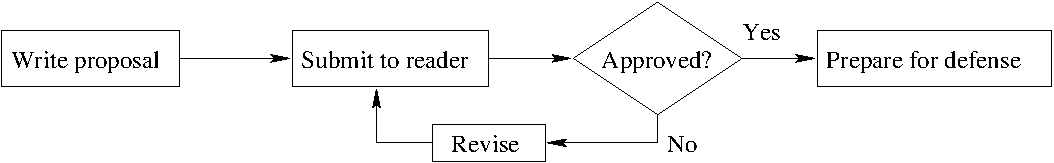
\includegraphics[width=5in]{flow.pdf}
  \caption{Flow graph for proposal-writing}~\label{intro-fig1}
\end{figure}

\begin{table}[htbp]
  \centering
  \begin{tabular}{|c||c|c|}
    \hline

    \bf Task     & \bf Begin Date & \bf End Date \\ \hline\hline
    First draft  & Now            & 20 Sept      \\ \hline
    Second draft & 20 Sept        & 27 Sept      \\ \hline
    Third draft  & 27 Sept        & 4 Oct        \\ \hline
    Fourth draft & 4 Oct          & 11 Oct       \\ \hline
    Fifth draft  & 11 Oct         & 18 Oct       \\ \hline

  \end{tabular}
  \caption{Illustrative Example of a Proposed Work Schedule}~\label{intro-tab1}
\end{table}

\section{Evaluation Strategy}
\label{sec:evaluate}

%   ********************************************************************
%   * Enter the text of your evaluation strategy section here.         *
%   ********************************************************************

Explain what steps you will take to evaluate your proposed method. If you intend
to conduct experiments, then you must clearly define your evaluation metrics.

\section{Research Schedule}
\label{sec:schedule}

Identify the main phases and tasks of your research project and set deadlines
for when you will be able to complete each of these items.

\section{Conclusion}
\label{sec:conclusion}

%   ********************************************************************
%   * Enter the text of your concluding section section here.          *
%   ********************************************************************

Provide a summary of your proposed research and suggest the impact that it may
have on the discipline of computer science. If possible, you may also suggest
some areas for future research.

\bibliographystyle{plain}
\bibliography{senior_thesis_proposal}

\end{document}
\grid
